\documentclass{article}
\usepackage{setspace}
\usepackage[utf8]{inputenc}



\usepackage{natbib}
\usepackage{graphicx}
\usepackage{amssymb} 
\doublespacing

\begin{document}
\begin{center}
  \large{JOHN JAY COLLEGE OF CRIMINAL JUSTICE}  \\
  \vspace{15mm}
  \large{MOBILE APPLICATION SECURITY}\\
  \vspace{15mm}
  \large{A THESIS SUBMITTED TO\\ THE CAPSTONE EXPERIENCE IN DIGITAL FORENSICS/CYBERSECURITY II}\\
  \large{IN CANDIDACY FOR THE DEGREE OF\\
BACHELOR’S IN COMPUTER SCIENCE AND INFORMATION SECURITY}\\
  \vspace{7mm}
  \large{DEPARTMENT OF COMPUTER SCIENCE}\\
  \vspace{15mm}
  \large{BY AHSAN KHAN}\\
   \vspace{15mm}
  \large{NEW YORK, NY}\\
  \large{02/01/2021 - 05/15/2021}
  \vspace{100mm}
\end{center}
\begin{center}
    \textbf{PLAGIARISM STATEMENT}
\end{center}
I know that plagiarism means taking and using the ideas, writings, works, or inventions of another as if they were one’s own. I know that plagiarism not only includes verbatim copying, but also the extensive use of another person’s ideas without proper acknowledgment (which includes the proper use of quotation marks). I know that plagiarism covers this sort of use of material found in textual sources and from the Internet. I acknowledge and understand that plagiarism is wrong. I understand that my research must be accurately referenced. I have followed the rules and conventions concerning referencing, citation and the use of quotations as set out in the Departmental Guide. This assignment is my work, or my group’s unique group assignment. I acknowledge that copying someone else’s assignment, or part of it, is wrong and that submitting identical work to others constitutes a form of plagiarism. I have not allowed, nor will I in the future allow anyone to copy my work to pass it off as their work. I certify that this thesis is my work, based on my study and research and that I have acknowledged all materials and sources used in its preparation, whether they be books, articles, reports, lecture notes, and any other kind of document, electronic or personal communication. The words quoted are from published and unpublished sources which are indicated and acknowledged as such. I also certify that this thesis has not previously been submitted for assessment in any other unit, except where specific permission has been granted from all unit coordinators involved, or at any other time in this unit, and that I have not copied in part or whole or otherwise plagiarized the work of other students or persons. As a member of a team project, I have only shared my knowledge with my team members, and have not let anyone copy my paper, nor I have copied any of their paper.\\
\vspace{100mm}
\begin{center}
    \textbf{ABSTRACT}
\end{center}
This paper is going to focus on Mobile Application Security, and how we can make our day-to-day experience a lot secured. We see and hear a lot about websites getting hacked and breached, but we never really pay attention to the mobile-specific breaches. As the world is evolving around mobile applications, it was become more important to focus on mobile application integrity, confidentiality, and availability. This research paper is highly based on the data security of the mobile application, and what steps a consumer and manufacturer can take to keep the data in a zone of CIA triad. For us to understand the importance of mobile application security, we will first need to know the background information of the major mobile manufacturer. It is also crucial for us to understand the applications that we download from these mobiles, and who publishes those applications. To talk about the security in mobile applications, we will start by talking about some past examples, and how they could have been avoided. Last but not the least, a security practitioner should know the tools like Kali Linux, penetration testing, etc, to combat mobile application breaches. Likewise, a user should also take the necessary steps to fulfill the best experience. The paper will also include the knowledge, skills, and abilities I learned in this project. There will be a cartoonish diagram that will show the secure password method and how to conduct a penetration test.
\vspace{100mm}
\tableofcontents
\vspace{100mm}
\section{Introduction}
What is application security? As the number of mobile devices increases every year, the idea of mobile security becomes more important than ever. Mobile Application Security is the protection of portable devices from threats, vulnerabilities, breaches, data being compromised, etc. When we talk about mobile security, we are usually talking about smartphones (Apple, Samsung, etc), tablets, smartwatches, e-reader, and you name it. People are now commonly using mobile devices for tasks that involve classified data like credit card numbers, social security numbers, and important banking information. Mobile application security is also about the practice of secure coding. Many breaches happen due to insecure coding practices. Internet and applications were not made by keeping security in mind, that’s why developers do not put much time on secure development, rather they would spend more time on UI/UX and make the application interactive. One quick teaser of a vulnerable mobile application is the use of a smartwatch to pay for things. Imagine you do not have a password on your apple pay/android pay, or you forgot to close the application, a knowledgeable threat actor would take full benefit of it by using the smartwatch to tap on his device and make your card pay for their things. According to the Federal Reserve, 39\% of all mobile phone users are using banking, up from 29\% in 2012. This would attract a lot of bad people, as they would be triggered to steal or manipulate your data. Some top issues are facing mobile devices, some that we will discuss in this paper are: Physical security, secure data storage, update process, spyware, multifactor authentication, safe browsing environment, and much more.
\vspace{100mm}
\section{What Are Mobile Applications/Manufacturers?}
According to techopedia, “A mobile application, most commonly referred to as an app, is a type of application software designed to run on a mobile device, such as a smartphone or tablet computer. Mobile applications frequently serve to provide users with similar services to those accessed on PCs. Apps are generally small, individual software units with limited function. This use of app software was originally popularized by Apple Inc. and its App Store, which offers thousands of applications for the iPhone, iPad, and iPod Touch. A mobile application also may be known as an app, web app, online app, iPhone app, or smartphone app.” \\
Two of the leading mobile manufacturers are Apple and Samsung. Apple’s smartphones use an operating system called iOS. iOS is considered as a closed source operating system, which means nobody would have access to the code, except the authorized developers of the iOS who are working for Apple. The advantages of having a closed source OS are that there is less confusion for customers, a unified experience, more security to the user, and more profit. On the other hand, Samsung uses an operating system called Android. Android OS is owned by Google, and there are many mobile manufacturers out there who rely on Android, except Apple. Android is an open-source OS, which means Google would release the code of the OS, and each manufacturer would have an option to modify the OS depending on their needs. The advantages of making an open-source OS are larger developer support, more secure as many developers around the world could read the code and find bugs in it, etc. One disadvantage of having an open-source model is that, if there is a bug that has not been found by a good developer, then a bad guy would use it to harm others. We call this 0-day vulnerability, as the vulnerability was never found before/brand new bug.
\vspace{100mm}
\section{Top Mobile Applications/The Process Of Uploading An Application}
How great would it be for the hackers to make a malicious application and submit it on the Apple app store and Android Play Store? Anyone who would download that malicious application will get infected, it is a win-win situation for the attacker. When it comes to security, Apple does not joke about it. The Apple applications are usually written in Swift and Objective-C. Anyone can go and learn these programming languages and make their application, but not everyone can submit the application on the app store. When it comes to submitting an application on the Apple app store, Apple would want you to confirm your identity, pay for the developer profile, and wait for 1-2 weeks for them to approve your applications. In that 1-2 weeks, the security team at Apple would run a security check on the application that you made and would look for hidden viruses or malware. They would also see the content of your application and if you have followed the secure coding practices. On the other hand, Android applications are written in Java or Kotlin. Android is more of a best friend for new developers, as they don’t have to pay anything to publish their applications, no security check, you can just make an account and publish your app.\\
The question is, how can a hacker harm you if you download a bad application on your smartphone. Let's say you download an application, the application requires you to input your full name, date of birth, address, phone number, and email, etc. Moving on they ask you to choose a security question, in case you forget your login information. For the security questions, you chose your mother’s maiden name, the first car bought, pet name, etc. Now lets imagine that the application is a gaming application and it has in-store purchase, for that you give your credit card or banking information. Now let us go back and see what happened.

 \begin{itemize}
   \item[$\blacksquare$] The attacker has your identity, he can make fake profiles with that.
   \item[$\blacksquare$] You gave the attacker the answer to your security questions that you would use on other applications, too. Now the attacker would try using this data to reset passwords on other platforms.
   \item[$\blacksquare$] You gave the attacker your banking information, now the attacker can make legal or illegal purchases with your money.
 \end{itemize}

Hypothetically speaking, what if applications like Instagram, Whatsapp, Netflix were to come from bad guys? Millions of people’s data would have been compromised by now. They will get compromised, but with some other methodologies.\\

\section{Example Of The Latest Mobile Application Security Breach}
According to Forbes, “The phone numbers and email addresses of 533 million Facebook users have been exposed in a data breach. Over the weekend, it emerged that the details of 533 million Facebook users, including phone numbers and email addresses passwords, had been leaked online. Facebook claims this data is from an old breach that took place in 2019. But now the information has been made widely available in a hacking forum online, it could potentially have been accessed by anyone.” Did they say emails and passwords? Does it mean that the attacker now can access my account, and in some cases may change my password, too? For us to understand the importance of having a strong password, let us first talk about some ways a company would choose to save your password.\\
When we set a password on your applications, the owner of the application has an option to save the password in multiple ways.\\

\begin{itemize}
   \item If your password is iloveyou, the company might save your password just in plain English, and it would look something like this => <username@email.com>: iloveyou. If I attack the database and I see your password, then I can simply log in to your account. That’s how FACEBOOK SAVED your passwords.
   \item If you set your account password as iloveyou, and the application owner decides to put some encryption on your password, then this is how it would look like after being encrypted \\
   =\textgreater \textless username@email.com\textgreater:\\ pTM4tJkf1DcVmCVzQMxWZ94NtTM8230wN/UQIVyo/U0=.\\ If I hack the database, this is the password that I will see. Note, encryption is reversible. This means, I can still crack this password using some brute force methodology or if I get access to the key.
   \item 	Lets say a company cares about their users, then they would use hashing to secure the passwords of their users. This is how a hashed password iloveyou would look like =\textgreater \textless username@emai.com\textgreater:\\ 50e0dc4455bcb1ee80adb942d153c6b0eb17b31d603b017fa77f60f60f68fd7d0\\565cb486783f29cea210313c97f0f9d49e64e6730053bfa1448d5b826309184.\\ Hashes are irreversible, means once a password is hashed, there is no way you can do reverse engineering to find the password or crack the hash. In this scenario, an attacker would make a list of all the common passwords, and then he will hash it. Then the attacker would compare the hash with this hash, if it matches, they find the password. The list where we save all the hashed passwords to compare them with other hashes, we call it a Rainbow Table.
   \item You might be thinking that there is no way for a company to secure your password. Actually, there is a way! We call this Salting the hash. This means if your password is iloveyou, the company would add random characters before or/and after the password, something like this “abciloveyouxyz”, and then they will hash this and store it. The characters “ABC XYZ” are the salt that they added to our password. Now if an attacker hacks the database and gets access to all the hashed passwords, there will be no way for the attacker to crack the hash, because the password they have in their rainbow table is just iloveyou, they do not know what characters we added to salt the passwords.
 \end{itemize}

\begin{figure}[h!]
\centering
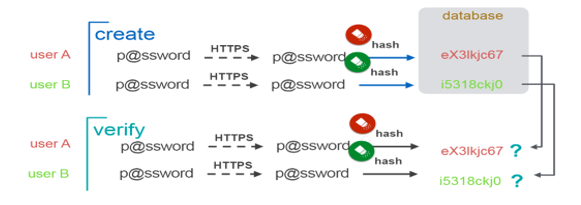
\includegraphics[]{fig.PNG}
\end{figure}
Why would a company like Facebook store our passwords in plain text? The answer is, we do not know. The assumptions can be weak security team, developers not educated on the security topics, etc. What can we as a user do to help ourself? Since we do not have access to the Facebook database, and there is no way we can do something about it, the best thing we can do is, just avoid using the same passwords for every application. Do not use the same password like Facebook, for the Chase Bank application.\\
\vspace{150mm}
\section{Tools That Can Be Used To Conduct A Mobile Application Security Audit}
As a  security practitioner, there are tools that a security team should use to conduct a complete security audit on the mobile application. Some tools are:\\

\begin{itemize}
   \item Encryption/Hashes/Cryptography
   \begin{itemize}
       \item To secure passwords, data, conversation, etc.
   \end{itemize}
   \item OWASP Mobile top ten
   \begin{itemize}
       \item A list for the developers' team to focus on when writing a code for a mobile application
   \end{itemize}
   \item Penetration testing
   \begin{itemize}
       \item Conduct a legal mobile application penetration testing to check the security of the application
   \end{itemize}
   \item Brute force attack
   \begin{itemize}
       \item Attack the account with millions of passwords, and check if there is any logical statement that would ban the IP after typing in the wrong password more than 5 times.
   \end{itemize}
   \item Ports and protocols being used in the mobile application
   \begin{itemize}
       \item What port(s) is the application using to transfer the data, is it secured?
   \end{itemize}
   \item Cloud security
   \begin{itemize}
       \item The data we save in dropbox, iCloud, is safe and secured, and encrypted?
   \end{itemize}
   
 \end{itemize}
\subsection{Cryptography / Hashes}
“With database encryption, an encryption algorithm transforms data within a database from a readable state into a ciphertext of unreadable characters. With a key generated by the algorithm, a user can decrypt the data and retrieve the usable information as needed.” In the security audit task, we can go deep into the database and see if the REST data is encrypted and stored securely. Encryption is reversible, so it is important to see how a company stores the key that would be used to decrypt the data.\\
“Hashes are the output of a hashing algorithm like MD5 (Message Digest 5) or SHA (Secure Hash Algorithm). These algorithms essentially aim to produce a unique, fixed-length string – the hash value, or “message digest” – for any given piece of data or “message”. As every file on a computer is, ultimately, just data that can be represented in binary form, a hashing algorithm can take that data and run a complex calculation on it and output a fixed-length string as the result of the calculation.” If the company is storing passwords on their database, it would worth every minute if a security audit team sees if the password is being salted and hashed or if it is just being saved as plain text.\\
\vspace{100mm}
\subsection{OWASP Mobile Top Ten}
“A comprehensive manual for mobile app security testing and reverse engineering for iOS and Android mobile security testers as well as developers. The OWASP Mobile Security top 10 is created to raise awareness for the current mobile security issues.” What are the top 10 issues listed on OWASP?\\
-	Improper platform usage\\
-	Insecure data storage\\
-	Insecure communication\\
-	Insecure authentication \\
-	Insufficient cryptography\\
-	Insecure authorization\\
-	Client code quality\\
-	Code tampering\\
-	Reverse engineering\\
-	Extraneous functionality\\
Make a list of the OWASP mobile top ten, briefly describe why it is important, and hand a copy to the developer team and the security. An application should never get published if it has even 1 thing from the list. Note, this list is not everything, these are just the top priorities.\\
\subsection{Penetration Testing}
A Mobile Application Penetration Test is an authorized and simulated hacking attempt against a native mobile application such as Android, Windows, and iOS. The purpose of this test is to identify and exploit vulnerabilities in an application, and the way it interacts and transfers data with the backend systems. A knowledge expert would use a list of OWASP's top ten, to first find the major vulnerabilities and trying to exploit them. Report the data exposure, if any. What insecure ports and protocols were being used, etc.\\
\subsection{Brute Force Attack}
“A brute force attack uses trial-and-error to guess login info, encryption keys, or find a hidden web page. Hackers work through all possible combinations hoping to guess correctly.” This step should be taken in the mobile application pen-test. An authorized pen-tester should conduct a brute force attack on the password, and see if the app allows trying as many passwords as you like. For best practice, disable the account after 5 tries and ban the IP until the case has not been resolved.\\
\subsection{Cloud Security}
Who does not run out of space on their phone, and then decide to save pictures, data, other stuff to iCloud or Dropbox or other cloud services. What do we know about them? Are they using the CIA triad on our data? There are many cloud services out there that you can use to save your data, but so many of them are not encrypting your data. When you save your Whatsapp chat to the cloud, they notify you that the chat is not encrypted. To pass an application in the security audit, it must become a priority to check if the data saved in the cloud is safe and encrypted. As many people are switching to cloud platforms, it has become more important than before to focus on cloud applications, too.\\
\vspace{100mm}
\section{KSA}
\textbf{Knowledge:} The path of writing this paper made me educate myself a lot on security topics. The number of research conducted, the videos I watched on youtube, the pen-test program at HackerOne, this all helped me increase my knowledge in the security field; especially mobile application security.\\
\textbf{Skills:} The number of skills I developed during this paper will help me lifelong. The biggest skill that I have achieved is to teach myself and make myself available to learn more. The technical skills that I have learned for this project are Kali Linux, Metasploit, Networking Protocols, iOS Development, Wireshark, Swift Language, LaTex, Penetration Testing, and much more.\\
\textbf{Abilities:} With the knowledge and skills that I have gained over this paper, I feel confident to write a small iOS application and conduct security research on it. Things like secure coding, penetration testing, databases, etc.
\vspace{150mm}
\section{Conclusion}
To conclude this paper, I would like to give some user awareness to the people out there. Just like a company has a responsibility to keep your data safe, the same way you will need to take some steps to do the same. Use a strong password for all your applications. Use a password manager. Do not leave the device unlocked and unattended. Do not fall for phishing or malicious apps, educate yourself on security.

\end{document}
